\subsection{CRM}
\label{subsec:crm}

\paragraph{CRM}
\textbf{C}ombined \textbf{R}adar \textbf{M}ode --- Combines A-A search submodes:

\begin{itemize}
    \item \textbf{RWS} --- \textbf{R}ange \textbf{W}hile \textbf{S}earch,
    see \Cref{subsec:rws}
    \item \textbf{TWS} --- \textbf{T}rack \textbf{W}hile \textbf{S}can,
    see \Cref{subsec:tws}
\end{itemize}

Selected by default on FCR start-up. Reference \cref{fig:crmoverview}

\paragraph{Change CRM Submode}
\begin{itemize}
    \item \textbf{OSB 2} --- \textbf{Press}
    \item Or \textbf{TMS} --- \textbf{Right Long}
\end{itemize}

\begin{figure}[htbp]
    \centering
    \begin{tikzpicture}[auto, node distance=10mm,x=1mm, y=1mm, very thick,
        >={Latex[round]}
        ]
        
        \path[
            fill=color2!20,
            rounded corners,
        ] (-50,90) -- (50,90) -- (50,45) -- (-50,45) -- cycle;
        \node[
            anchor=north west,
        ](mark)at(-50,90){\scriptsize \blue{Supports AIM-120 Launch}};
        \path[
            fill=color2!60,
            rounded corners,
        ] (-47.5,85) -- (0,85) -- (0,90) -- (50,90) -- (50,75) -- (-47.5,75) -- cycle;
        \node[
            anchor=north east,
        ](mark)at(50,90){\scriptsize \textbf{\color{white}RWR Launch Warning}};
        % \node[<options>](<coordinate name>)at(<coordinate>){<text>};
        \node[
            hyperref node=subsec:rws,
            rectangle,
            rounded corners,
            minimum width=15mm,
            minimum height=15mm,
            draw,
        ](rws)at(0,0){\blue{RWS}};
        \node[
            rectangle,
            rounded corners,
            minimum width=25mm,
            minimum height=7.5mm,
            draw,
            fill=white,
        ](sam)at(0,50){\textbf{SAM}};
        \node[
            rectangle,
            rounded corners,
            minimum width=25mm,
            minimum height=7.5mm,
            draw,
            fill=white,
        ](dtt)at(-32.5,65){\textbf{DTT}};
        \node[
            hyperref node=subsec:tws,
            rectangle,
            rounded corners,
            minimum width=15mm,
            minimum height=15mm,
            draw,
        ](tws)at(32.5,0){\blue{TWS}};
        \node[
            rectangle,
            rounded corners,
            minimum width=25mm,
            minimum height=7.5mm,
            draw,
            fill=white,
        ](systgt)at(32.5,20){\textbf{System Tgt}};
        \node[
            rectangle,
            rounded corners,
            minimum width=25mm,
            minimum height=7.5mm,
            draw,
            fill=white,
        ](cursortgt)at(32.5,35){\textbf{Cursor Tgt}};
        \node[
            rectangle,
            rounded corners,
            minimum width=25mm,
            minimum height=7.5mm,
            draw,
            fill=white,
        ](bug)at(32.5,50){\textbf{Bugged}};
        \node[
            hyperref node=subsec:stt,
            rectangle, 
            rounded corners,
            minimum width=90mm,
            minimum height=7.5mm,
            draw, 
            fill=white,
        ](stt)at(0,80){\blue{STT}};
        
        % Lines
        \draw [->]
            (rws) -- node[pos=0.5, left]{\scriptsize\textbf{TMS FWD}} (sam);
        \draw [<->]
            (rws) -- node[pos=0.5, above]{\scriptsize\textbf{TMS RIGHT}}node[pos=0.5, below]{\scriptsize\textbf{(long)}} (tws);
        \draw [->, rounded corners]
            (sam) -| node[pos=0.25, above]{\scriptsize\textbf{TMS FWD}}node[pos=0.25, below]{\scriptsize\textbf{(2nd Tgt)}} (dtt);
        \draw [->]
            (tws) -- node[pos=0.5, left]{\scriptsize\textbf{TMS FWD}} (systgt);
        \draw [->]
            (systgt) -- node[pos=0.5, left]{\scriptsize\textbf{Cursor Over}} (cursortgt);
        \draw [->]
            (cursortgt) -- node[pos=0.5, left]{\scriptsize\textbf{TMS FWD}} (bug);
        \draw [->]
            let
                \p1=(dtt.north),
                \p2=(stt.south)
            in
                (\p1) -- node[pos=0.5, left]{\scriptsize\textbf{TMS FWD}} (\x1,\y2);
        \draw [->]
            let
                \p1=(sam.north),
                \p2=(stt.south)
            in
                (\p1) -- node[pos=0.5, left]{\scriptsize\textbf{TMS FWD}}node[pos=0.5, right]{\scriptsize\textbf{(1st Tgt)}} (\x1,\y2);
        \draw [->]
            let
                \p1=(bug.north),
                \p2=(stt.south)
            in
                (\p1) -- node[pos=0.5, left]{\scriptsize\textbf{TMS FWD}} (\x1,\y2);
    \end{tikzpicture}
    \caption{CRM Radar Modes Overview}
    \label{fig:crmoverview}
\end{figure}

\clearpage

\subsubsection{A-A SEARCH SCAN PATTERN}

\paragraph{Radar Gimbal Limits}
APG-68 is mechanically scanned on 2 axis gimbal
\begin{itemize}
    \item \textbf{Azimuth} --- \pm60 deg (120 deg coverage)
    \item \textbf{Vertical} --- \pm60 deg (120 deg coverage)
\end{itemize}

\paragraph{Azimuth Scan Pattern}
Horizontal scan volume controlled by selecting limits of gimbal azimuth
\begin{itemize}
    \item \textbf{Azimuth search patterns}
    \begin{itemize}
        \item \textbf{A6} --- \pm60 deg
        \item \textbf{A3} --- \pm30 deg (centered on cursor)
        \item \textbf{A1} --- \pm10 deg (centered on cursor)
    \end{itemize}
    \item \textbf{Cycled via}
    \begin{itemize}
        \item \textbf{OSB 18} cycles available azimuth patterns
        \item walking cursor off side of FCR display in RWS cycles A6/A3
    \end{itemize}
    \item \textbf{TWS \& DTT modes use a special \pm25 deg,
    3 bar scan pattern}
    \begin{itemize}
        \item \textbf{A2} --- \pm25 deg (centered on cursor / target)
    \end{itemize}
\end{itemize}

Reference \cref{fig:sensors_aa:apg68:crm:azscan} for graphical representation

\paragraph{Bar Scan Pattern}
Elevation scan volume controlled by selecting number of ``bars'' (horizontal sweeps)
\begin{itemize}
    \item \textbf{B4} / \textbf{B2} / \textbf{B1} --- cycled via \textbf{OSB 17}
    \item \textbf{B3} --- selected by TWS \& DTT modes
\end{itemize}

Reference \cref{fig:sensors_aa:apg68:crm:barscan} for graphical representation

\begin{figure}[htbp]
    \centering
    \begin{tikzpicture}[auto, node distance=10mm, x=1mm, y=1mm, very thick, line cap=round,
        >={Latex[round]}
        ]

        \node[
            anchor=east
        ] (mfd) at (0,0) {
            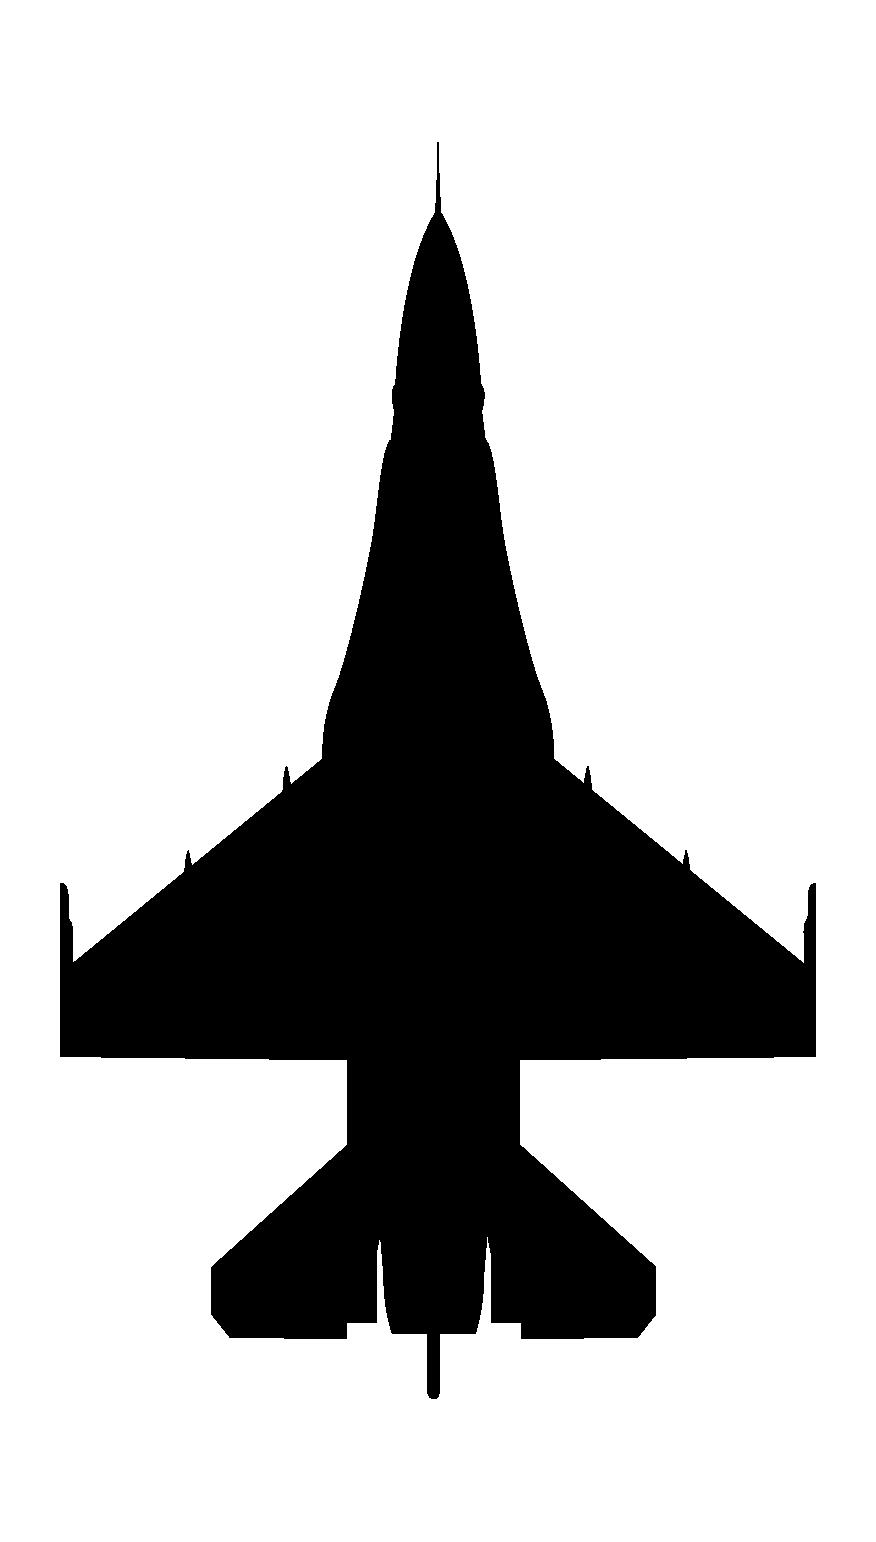
\includegraphics[
                height=15mm,
                angle=-90,
            ]{diagrams/aircraft/silhouette_f16_top.pdf}
        };

        \coordinate (offset) at (-3.5,0);
        \coordinate (center) at ($(offset)+(0:38)$);

        \draw[]
        (offset) -- node[pos=1, above right, font=\small\bfseries] {A6} +(60:30) arc (60:-60:30) -- cycle;
        \draw[]
        (offset) -- node[pos=1, above right, font=\small\bfseries] {A3} +(30:32) arc (30:-30:32) -- cycle;
        \draw[]
        (offset) -- +(25:34) arc (25:-25:34) -- node[pos=0, right, font=\small\bfseries] {A2} cycle;
        \draw[]
        (offset) -- node[pos=1, right, font=\small\bfseries] {A1} +(10:36) arc (10:-10:36) -- cycle;
        \draw[color2, fill=color2!20]
        (offset) -- +(1.5:38) arc (1.5:-1.5:38) -- cycle;

        \node[anchor=west, align=left, font=\small\bfseries, color2] at (center) {BEAMWIDTH};
    \end{tikzpicture}
    \caption{
        FCR azimuth scan \& limits. 
        Note that the A6 pattern scans the entire azimuth range of the radar.
        The varying radii for the different azimuth settings are for illustrative purposes.
    }
    \label{fig:sensors_aa:apg68:crm:azscan}
\end{figure}

\begin{figure}[htbp]
    \centering
    \begin{tikzpicture}[auto, node distance=10mm, x=1mm, y=1mm, very thick, line cap=round,
        >={Latex[round]}
        ]

        \node[
            anchor=east
        ] (mfd) at (0,0) {
            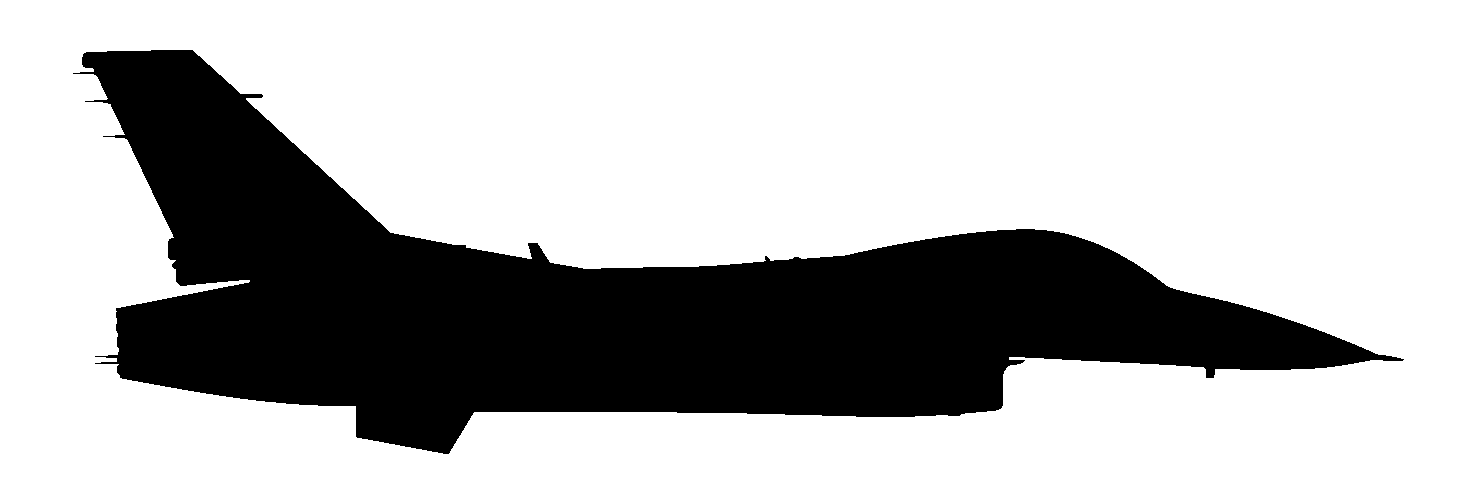
\includegraphics[
                width=15mm,
            ]{diagrams/aircraft/silhouette_f16_side.pdf}
        };

        \coordinate (offset) at (-2.5,-1);
        \coordinate (4bar) at ($(offset) + (36:35)$);
        \coordinate (3bar) at ($(offset) + (12:35)$);
        \coordinate (2bar) at ($(offset) + (-12:35)$);
        \coordinate (1bar) at ($(offset) + (-36:35)$);

        \node[font=\small\bfseries] at ($(4bar)+(5,2.5)$) {4B};
        \node[font=\small\bfseries] at ($(3bar)+(5,0)$) {3B};
        \node[font=\small\bfseries] at ($(2bar)+(5,0)$) {2B};
        \node[font=\small\bfseries] at ($(1bar)+(5,-2.5)$) {1B};

        \draw[]
        (offset) -- node[pos=1, above, font=\small\bfseries] {+/- 60 deg} +(60:35) arc (60:-60:35) -- cycle;
        \draw[color2, fill=color2!20]
        (offset) -- +(41.75:35) arc (41.75:31.25:35) -- cycle;
        \draw[color2, fill=color2!20]
        (offset) -- +(16.65:35) arc (16.65:7.35:35) -- cycle;
        \draw[color2, fill=color2!20]
        (offset) -- +(-8.45:35) arc (-8.45:-15.55:35) -- cycle;
        \draw[color2, fill=color2!20]
        (offset) -- +(-33.55:35) arc (-33.55:-38.45:35) -- cycle;

        \coordinate (4boffset) at ($(4bar) + (15,2.5)$);
        \coordinate (3boffset) at ($(3bar) + (15,0)$);
        \coordinate (2boffset) at ($(2bar) + (15,0)$);
        \coordinate (1boffset) at ($(1bar) + (15,-2.5)$);

        % 4bar
        \filldraw[color2!20] ($(4boffset) + (22.5,3.75)$) circle (2.5);

        \draw[->, rounded corners, ultra thick,]
        (4boffset)
        -- ($(4boffset) + (0,3.75)$)  -- ($(4boffset) + (20,3.75)$);
        \draw[->, rounded corners, ultra thick,]
        ($(4boffset) + (20,3.75)$)
        -- ($(4boffset) + (40,3.75)$) -- ++(0,-2.5)
        -- ++(-39,0) -- ++(0, -2.5)
        -- ++(39,0) -- ($(4boffset) + (+40,-3.75)$)
        -- ($(4boffset) + (20,-3.75)$);
        \draw[rounded corners, ultra thick,]
        ($(4boffset) + (20,-3.75)$)
        -- ($(4boffset) + (0,-3.75)$) 
        -- (4boffset);

        \draw[dashed, rounded corners=5]
        ($(4boffset) + (-2.5,6.25)$) -- ($(4boffset) + (42.5,6.25)$)
        -- ($(4boffset) + (42.5,-6.25)$) -- ($(4boffset) + (-2.5,-6.25)$)
        -- cycle;

        \draw[color2, ultra thick] ($(4boffset) + (22.5,3.75)$) circle (2.5);

        % 3bar
        \draw[->, rounded corners, ultra thick,]
        ($(3boffset) + (2.5,0)$) -- (3boffset)
        -- ($(3boffset) + (0,2.5)$) -- ($(3boffset) + (20,2.5)$);
        \draw[->, rounded corners, ultra thick,]
        ($(3boffset) + (20,2.5)$)
        -- ($(3boffset) + (40,2.5)$) -- ++(0,-2.5)
        -- ($(3boffset) + (20,0)$);
        \draw[->, rounded corners, ultra thick,]
        ($(3boffset) + (20,0)$)
        -- ($(3boffset) + (0,0)$) -- ++(0, -2.5)
        -- ($(3boffset) + (+20,-2.5)$);
        \draw[rounded corners, ultra thick,]
        ($(3boffset) + (+20,-2.5)$)
        -- ($(3boffset) + (+40,-2.5)$) -- ++(0,2.5)
        -- ($(3boffset) + (2.5,0)$);

        \draw[dashed, rounded corners=5]
        ($(3boffset) + (-2.5,5)$) -- ($(3boffset) + (42.5,5)$)
        -- ($(3boffset) + (42.5,-5)$) -- ($(3boffset) + (-2.5,-5)$)
        -- cycle;

        % 2bar
        \draw[->, rounded corners, ultra thick,]
        (2boffset)
        -- ($(2boffset) + (0,1.25)$) -- ($(2boffset) + (20,1.25)$);
        \draw[->, rounded corners, ultra thick,]
        ($(2boffset) + (20,1.25)$)
        -- ($(2boffset) + (40,1.25)$)
        -- ($(2boffset) + (40,-1.25)$) -- ($(2boffset) + (20,-1.25)$);
        \draw[rounded corners, ultra thick,]
        ($(2boffset) + (20,-1.25)$)
        -- ($(2boffset) + (0,-1.25)$)
        -- (2boffset);

        \draw[dashed, rounded corners=5]
        ($(2boffset) + (-2.5,3.75)$) -- ($(2boffset) + (42.5,3.75)$)
        -- ($(2boffset) + (42.5,-3.75)$) -- ($(2boffset) + (-2.5,-3.75)$)
        -- cycle;

        % 1bar
        \draw[->, rounded corners, ultra thick,]
        ($(1boffset) + (0,0)$) -- ($(1boffset) + (15,0)$);
        \draw[->, rounded corners, ultra thick,]
        ($(1boffset) + (40,0)$) -- ($(1boffset) + (25,0)$);
        \draw[rounded corners, ultra thick,]
        ($(1boffset) + (25,0)$) -- ($(1boffset) + (0,0)$);

        \draw[dashed, rounded corners=5]
        ($(1boffset) + (-2.5,2.5)$) -- ($(1boffset) + (42.5,2.5)$)
        -- ($(1boffset) + (42.5,-2.5)$) -- ($(1boffset) + (-2.5,-2.5)$)
        -- cycle;
    \end{tikzpicture}
    \caption{
        FCR elevation scan \& limits. 
        The radar beam --- blue circle --- tracks along the illustrated scan pattern in a loop, resulting in the dashed scan volume. 
        Note that the scan patterns are not drawn to scale.
    }
    \label{fig:sensors_aa:apg68:crm:barscan}
\end{figure}

\clearpage

\subsubsection{MFD CONTROLS}

\paragraph{Radar Mode}
\textbf{OSB 1} opens page allowing selection of radar mode
\begin{itemize}
    \item \textbf{Left Side (OSB 19-20)} --- A-A Modes
    \begin{itemize}
        \item CRM --- see \cref{subsec:crm}
        \item ACM --- see \cref{subsec:acm}
    \end{itemize}
    \item \textbf{Right Side (OSB 6-9)} --- A-G Modes
    \begin{itemize}
        \item see \cref{sec:fcr-ag}
    \end{itemize}
    \item \textbf{STBY (OSB 10)} --- places FCR in standby
\end{itemize}

\paragraph{Field of View}
\textbf{OSB 3} cycles field of view

\begin{itemize}
    \item \textbf{EXP} --- expanded field of view
    \item \textbf{NORM} --- normal field of view
\end{itemize}

HOTAS \textbf{EXPAND/FOV} switch also cycles FOV

\paragraph{Override} 
Pressing \textbf{OVRD (OSB 4)}  places FCR in standby

\paragraph{FCR Control} 
\textbf{CNTL (OSB 5)} opens FCR control page

\paragraph{Datalink Mode} 
\textbf{OSB 6} cycles datalink operating mode (WIP)

\paragraph{Declutter} 
\textbf{DCLT (OSB 11)} opens FCR declutter page,
allowing pilot to deselect symbology elements

\paragraph{Elevation Bar Select} 
\textbf{OSB 17} cycles elevation bar search pattern

\paragraph{Azimuth Select}
\textbf{OSB 18} cycles azimuth search pattern
\paragraph{Range Select}
\textbf{OSB 19-20} adjusts FCR display range scale

\begin{itemize}
    \item \textbf{Can be cycled by ``walking'' cursor off top/bottom of display}
\end{itemize}

\notebox{\small
    Azimuth and range can also be cycled by ``walking'' acquisition cursor off the side and top/bottom of FCR display respectively
}

\begin{figure}[htbp]
    \centering
    \begin{tikzpicture}[auto, node distance=10mm, x=1mm, y=1mm, very thick, line cap=round,
        >={Latex[round]}
        ]
        
        \node[] (fig) at (0,0) {
            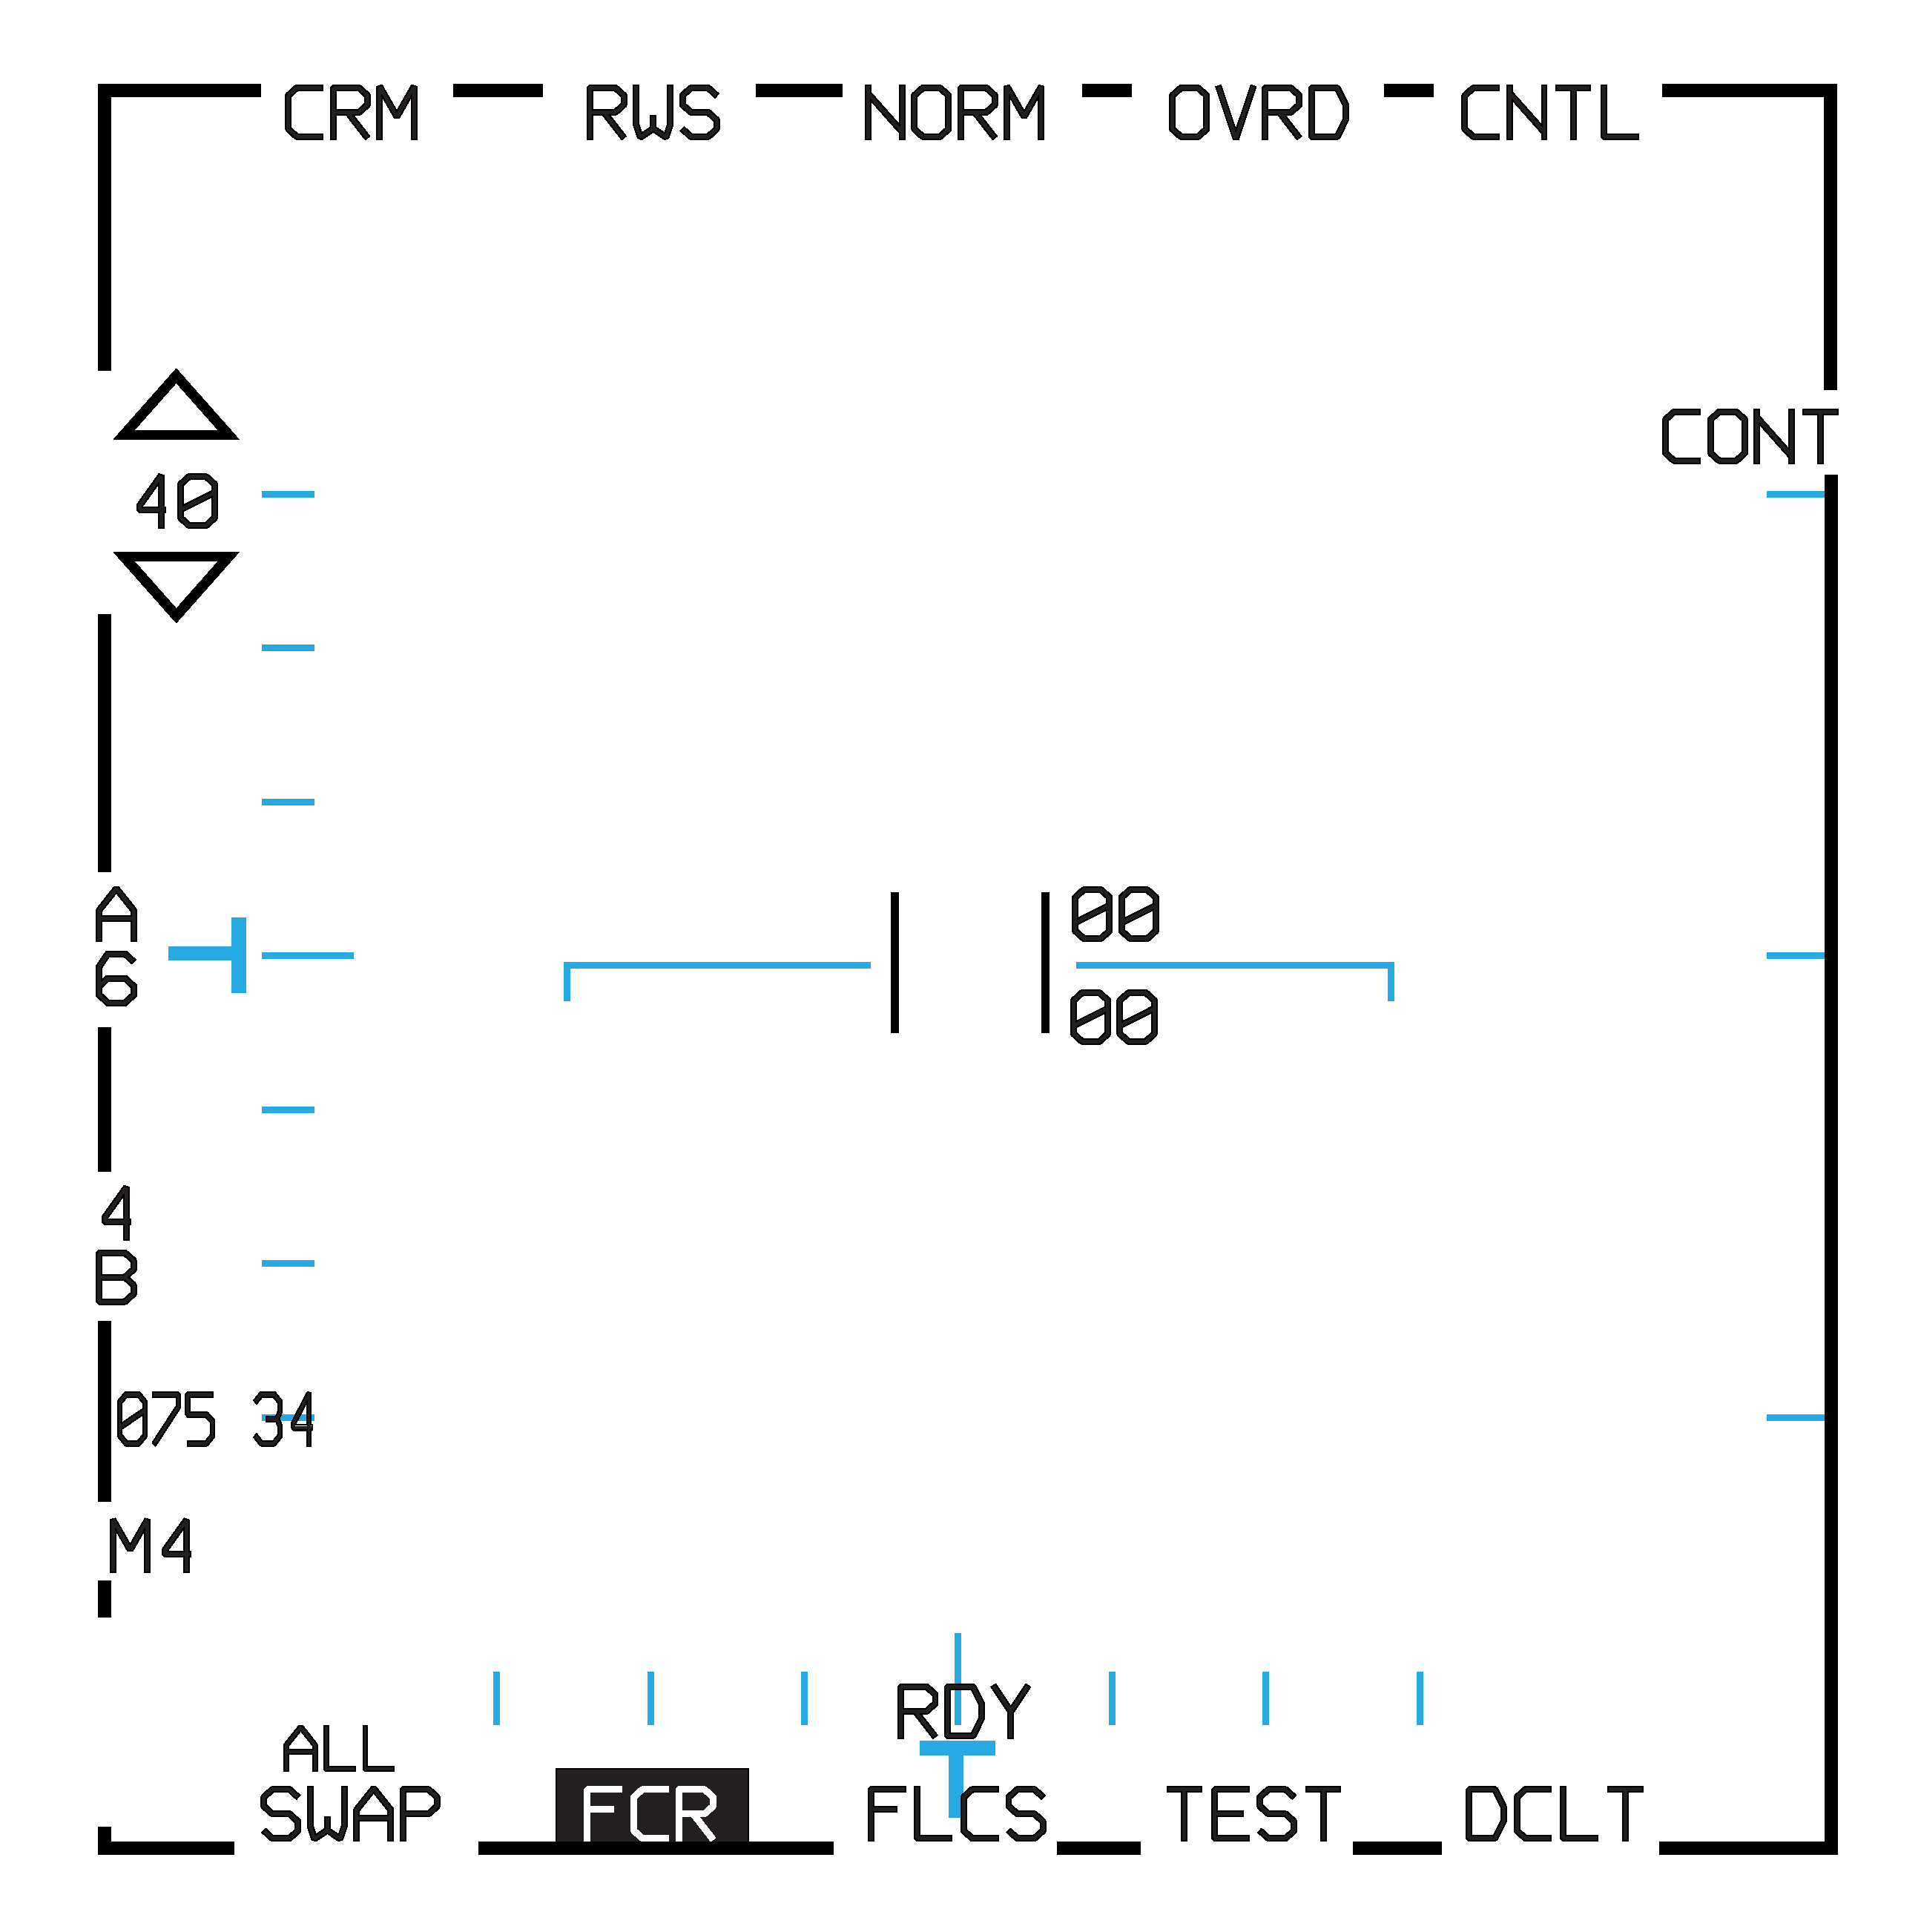
\includegraphics[
                height=75mm,
            ]{mfd/fcr_aa/rws_homepage.pdf}
        };

        % Annotations
        \node[lannot] (mode) at ($(fig.west)+(0mm,38mm)$) {FCR mode};
        \draw[annotptr] (mode.east) -- ++(12mm, 0mm) -- (-24mm,35mm);

        \node[lannot] (submode) at ($(fig.west)+(0mm,28mm)$) {CRM \\ submode};
        \draw[annotptr] (submode.east) -- ++(23mm, 0mm) -- (-13mm, 31mm);

        \node[lannot] (rsel) at ($(fig.west)+(0mm,18mm)$) {Range select};
        \draw[annotptr] (rsel.east) -- ++(4.5mm, 0mm);

        \node[lannot] (asel) at ($(fig.west)+(0mm,0.5mm)$) {Azimuth select};
        \draw[annotptr] (asel.east) -- ++(4.5mm, 0mm);

        \node[lannot] (bsel) at ($(fig.west)+(0mm,-10.5mm)$) {Elevation bar select};
        \draw[annotptr] (bsel.east) -- ++(4.5mm, 0mm);

        \node[annot, anchor=south, align=center] (fov) at ($(fig.north)+(0mm,0mm)$) {FOV select};
        \draw[annotptr] (fov.south) -- ++(0mm, -3.5mm);

        \node[rannot] (cntl) at ($(fig.east)+(0mm,38mm)$) {Control};
        \draw[annotptr] (cntl.west) -- ++(-13mm, 0mm) -- (23mm, 35mm);

        \node[rannot] (ovrd) at ($(fig.east)+(0mm,28mm)$) {Override};
        \draw[annotptr] (ovrd.west) -- ++(-24mm, 0mm) -- (12mm, 31mm);

        \node[rannot] (dl) at ($(fig.east)+(0mm,20.5mm)$) {Datalink mode};
        \draw[annotptr] (dl.west) -- ++(-4mm,0mm);

        \node[rannot] (acq) at ($(fig.east)+(0mm,10mm)$) {Acquisition cursor};
        \draw[annotptr] (acq.west) -- ++(-30mm, 0mm) -- (3mm,5mm);

        \node[rannot] (sj) at ($(fig.east)+(0mm,-8mm)$) {Horizon \\indicator};
        \draw[annotptr] (sj.west) -- ++(-20mm, 0mm) -- (12mm,-1mm);

        \node[rannot] (dclt) at ($(fig.east)+(0mm,-38mm)$) {Declutter};
        \draw[annotptr] (dclt.west) -- ++(-13mm, 0mm) -- (23mm, -35mm);
    \end{tikzpicture}
    \caption{FCR page with basic controls \& symbology marked. Note that FCR is illustrated in default mode immediately after startup.}
\end{figure}